\documentstyle[psfig,12pt,tabularx]{article}
\sloppy

\textheight 23cm
\textwidth 15cm
\leftmargin 4cm
\topmargin -1.5cm
\begin{document}
\pagestyle{empty}

\begin{center}
%{ \Huge The Roland Maze Project} 
 
\

\vspace{2cm}

{\huge Tadeusz Wibig}

 \vspace{1cm}
\noindent
{{\Large \it Experimental Physics Dept., University of \L \'{o}d\'{z}; 

\vspace{.3cm} \noindent
Cosmic Ray Lab.,  
The Andrzej So{\l }tan Institute for Nuclear Studies,  
{\L }\'{o}d\'{z} 1, P.O.Box 447, 
Poland}}
 
%\date{\today} 
 
%\draft 
 
\vspace{1cm}

%\maketitle 
 \Large
\begin{minipage}{15cm}
The project of the cosmic ray experiment involving high school
students (and teachers) could be of great importance not only because of its
eventual physical results but also can have a great impact on
the future of young people, introducing to them quite new and
unknown, in general, field of science. The idea is to build an array of cosmic
ray detectors distributed in the \L \'{o}d\'{z} area high schools, each
being autonomous small sub-array connected with others by the Internet.
Similar projects are at present in the R\&D phase in USA and Canada and it is
believed that they start collecting data (and experiences) in near future.
\end{minipage}    
\end{center}

\newpage
\Large
High energy ($E>10^{18}$eV) cosmic ray particles continuously strike the
Earth's atmosphere from outer space create avalanches of daughter particles
which cover the areas measured in square kilometers on the ground. The
important physical question: "where they come from?" is still unanswered. Even
the nature of these particles is unclear. They could be, in principle, 
protons, heavier nuclei, $\gamma$ quanta, neutrinos, or even undiscovered yet
in laboratory accelerator experiments new particles appearing in some theories
beyond the Standard Model. Studies of showers initiated by such objects is the
subject of huge experiments (like Auger Observatory, or OWL, to name only few)
of budgets beyond 100 ml \$. 

The problem is that such particles are extremely rare (see the figure). To
get reasonable statistic effective area of the apparatus should be measured
in km$^2$ (The biggest existing AGASA is of order of 100 km$^2$). Such an area
could not be filled continuously with detectors, thus (only?) the question of
money is how dense the detector net could be. Usually the spacing is of order
of 1 km.

\newpage
We propose to put the set of four detectors on each high school in the city 
(see the map) obtaining thus the network of quite reasonable size and
spacing. Each station will be able to determined the particle density of
shower particles and time of their arrival. For the timing purposes we would
like to use GPS system and for communication the Internet connection.

\newpage
For educational purposes each station will able to have its oven trigger and
timing system which allows students to study the CR spectrum, anisotropy and to
make some other interesting, small experiments and tests. 
Four detectors spacing of about 10 m will be installed of the roof of the
school together with the GPS antenna. The electronics will process
signals send them to the PC on which the data will be stored (and
pre-analyzed). The registrations will be from time to time send to the central
server where data from all stations (schools) will by stored and from each 
group will be able to load them upon request.

\newpage
To build the station network is only the one problem, another, may be even more
important to organize the serial of lectures for teachers (and students) which
will give them the knowledge needed to understand the
subject of their studies. It include the preparation of documentation and 
continuous monitoring of their activities during all phases of the experiment.
This is ambitious task, but we think that if we will try hard the results
could be very satisfactory to everyone.

\newpage
{\bf Roland Maze} 
together with Pierre Auger discovered extensive air showers using the small
apparatus he made on the roof of 
\'{E}cole Normale Sup\'{e}rieure is Paris in 1938. 

From '50 when our cosmic ray group starts their activities he
closely collaborate with physicists in {\L }\'{o}d\'{z}. His name
appear among the names of Aleksander Zawadzki,
 Juliusz
Hibner, Jerzy
 Gawinem, and Jerzy Wdowczyk in the number of
publications which make our laboratory significant in the
cosmic ray physics community.

Comparing the scale and aims of our project and the international Project
Auger it seems quite reasonable to call our project, to honor the great
physicist, the Roland Maze project.
\newpage
 


\newpage

%\begin{figure} 
\centerline{ 
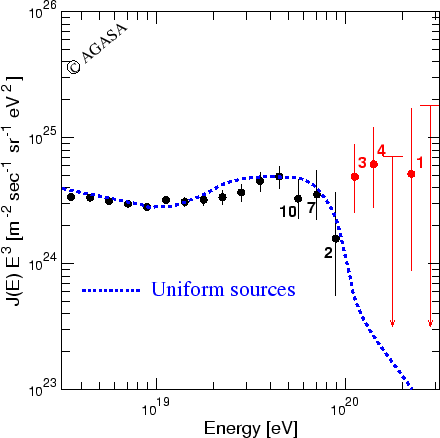
\psfig{file=spectrum.eps,width=15cm,angle=0}} 
%\caption
{Cosmic ray energy spectrum.} 
%\end{figure} 

\newpage

\begin{figure} 
\centerline{ 
\psfig{file=licea.eps,width=15cm,angle=0}} 
%\caption
{Map of high schools in \L \'{o}d\'{z}.} 
%\end{figure} 

%\begin{figure} 
\centerline{ 
\psfig{file=app1.eps,width=8cm,angle=0}} 
%\caption
{The view of detectors on the school roof.} 
%\end{figure} 

%\begin{figure} 
\centerline{ 
\psfig{file=app2.eps,width=8cm,angle=0}} 
%\caption{ 
Single detector: a - plastic scintillator, b - light fiber with wave-length
shifter, c - avalanche photo-diode.

%\end{figure} 

\end{document}


